\documentclass{article}
\usepackage[utf8]{inputenc}
\usepackage{romannum}
\usepackage{amsfonts}
\usepackage{amssymb}
\usepackage{fancyhdr}
\usepackage{graphicx}
\usepackage{t1enc}
\usepackage{pdfpages}
\usepackage[magyar]{babel}
\usepackage[utf8]{inputenc}
\usepackage{amsmath}
\usepackage{mathtools}
\usepackage{pdfpages}
\usepackage{ marvosym } 
\usepackage{wrapfig}
\usepackage{hyperref}
\usepackage{pgfplots}

\pgfplotsset{width=\textwidth,compat=newest}
\hypersetup{
    colorlinks,
    citecolor=black,
    filecolor=black,
    linkcolor=black,
    urlcolor=black
}
\usepackage{romannum}
\usepackage{amsfonts}
\usepackage{amssymb}
\usepackage{fancyhdr}
\usepackage{graphicx}
\usepackage{t1enc}
\usepackage{svg}
\usepackage[magyar]{babel}
\usepackage[left=2cm,right=2cm,top=2cm,bottom=2cm]{geometry}

\title{K+F Projekt dokumentáció}
\author{}
\date{2}
\pagestyle{fancy}
\lhead{K+F Projekt dokumentáció}
\rhead{ACSG Kft.}
\cfoot{\thepage. oldal}

\begin{document}
\pagenumbering{arabic}

\begin{center}
    \hrule
    \vspace{0.5cm}
    \begin{Huge}
    K+F projekt dokumentáció\\
    ACSG Kft.\\
    \end{Huge}
    \vspace{0.5cm}
    \begin{huge}
    Időszak:\\
    \end{huge}
    \begin{Large}
    2022.11.01. - 2022.12.31.\\
    \end{Large} \vspace{10pt}
    \begin{large}
    Készítette: Wenesz Dominik\\
    \end{large}\vspace{0.5cm}
    \hrule
    
  \end{center}
  \begin{figure}[b]
    \centering
    
\includegraphics[]{acsg.png}
\end{figure}

  


\thispagestyle{empty}
\setcounter{page}{0}




\newpage
\tableofcontents
\newpage

\section{Összefoglaló}
A dokumentum által specifikált időintervallumban a detektáló rendszerben történtek
főbb előrelépések. Először is a későbbi skálázhatóságra való tekintettel hardveres
területen változtattunk a feldolgozó egységet és kamerarendszert illetőleg. 
Ezenfelül a hagyományos képfeldolgozási módszerek után a mélytanuláson alapuló
módszerek applikálhatóságát vizsgáltuk.\\
A másik terület, melyben munkálatok folytak, az a manipulátor megfogójának
milyenségének kiválasztása, többféle csatlakozóházon való tesztelése. Ez explicit
nem a robotkar pontosságának mérését jelenti, hanem a kereskedelemben fellelhető
végberendezések egymással való összehasonlítását (pl.: strapabíróság, felvehető objektum paraméterei, felvehető objektumok számossága, objektumdetektáló rendszerre 
való illeszthetősége, stb.). A robot pontosságának vizsgálata a következő két hónapos
indőintervallumra esedékes.

\section{Objektum detektáló alrendszer}
\subsection{Hardver változtatások}
Az objektum detektálás szempontjából a Jetson Nano és a RaspberryPi V2.1-es kamera
elegendőnek tekinthető, azonban azon megfontolásból, hogy a későbbiekben 
a rendszer bővíthető legyen, esetlegesen párhuzamosan több feladatot is el
tudjon látni, például egyszerre több különálló kamerakép alapján több 
egymástól független párhuzamos program/algoritmus futhasson párhuzamosan valós
időben, vagy egy komplex, egész gyártócellára kiterjedő optimalizációs rendszer
is futtaható legyen, arra a konklúzióra jutottunk, hogy egy nagyobb erőforrásokkal
rendelkező feldolgozó egységet használunk. Így esett a választás a Jetson Xavier NX-re,
melynek adatlapja megtalálható mellékelve a dokumentációs mappában.\\[5pt]
\begin{figure}[h]
    \centering
    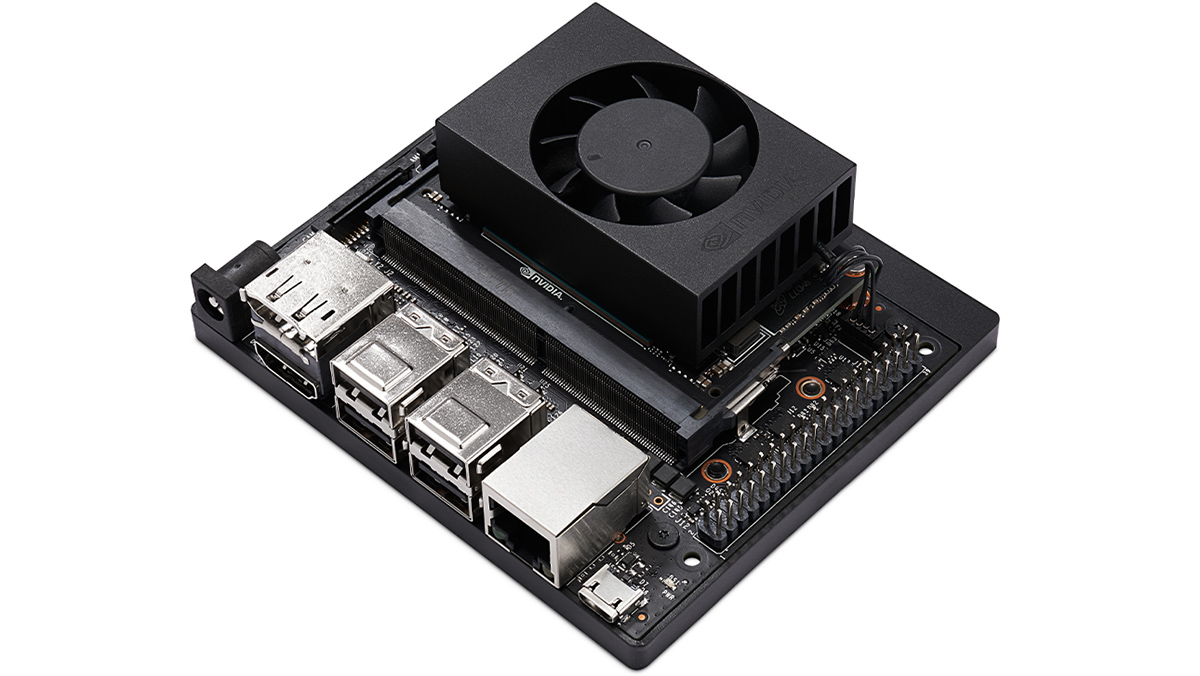
\includegraphics[scale=0.3]{xavier.jpg}
    \caption[]{Jeston Xavier NX Edge System}
\end{figure}\\
Ezen modul előnye, hogy több memóriát, nagyobb számítókapacitású CPU-t és 
nagyobb teljesítményű GPU-t tartalmaz, melyek amint azt későbbiekben láthatjuk 
a mélytanulásos objektumdetektáló módszerekhez elengedhetetlenek.\\[15pt]
A kamera modul választásában szintén változtattunk, mivel a RPi V2.1 képminősége
a kisebb objektumoknál már nem bizonyult megfelelőnek, illetve nem bővíthető
gyárilag lencserendszerrel, így precíz hangolása nehézkes. Ezen indokoknál
fogva választottuk a RaspBerryPi HQ detektort a hozzá tartozó lencserendszerrel 
(optikával) együtt, melyet könnyedén tudunk precízen hangolni. A szenzor és az 
optika adatlapja szintén megtalálható a dokumentáció megfelelő almappájában.\\[5pt]
\begin{figure}[h]
    \centering
    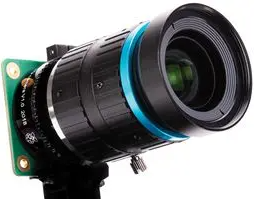
\includegraphics[scale=1]{optika.png}
    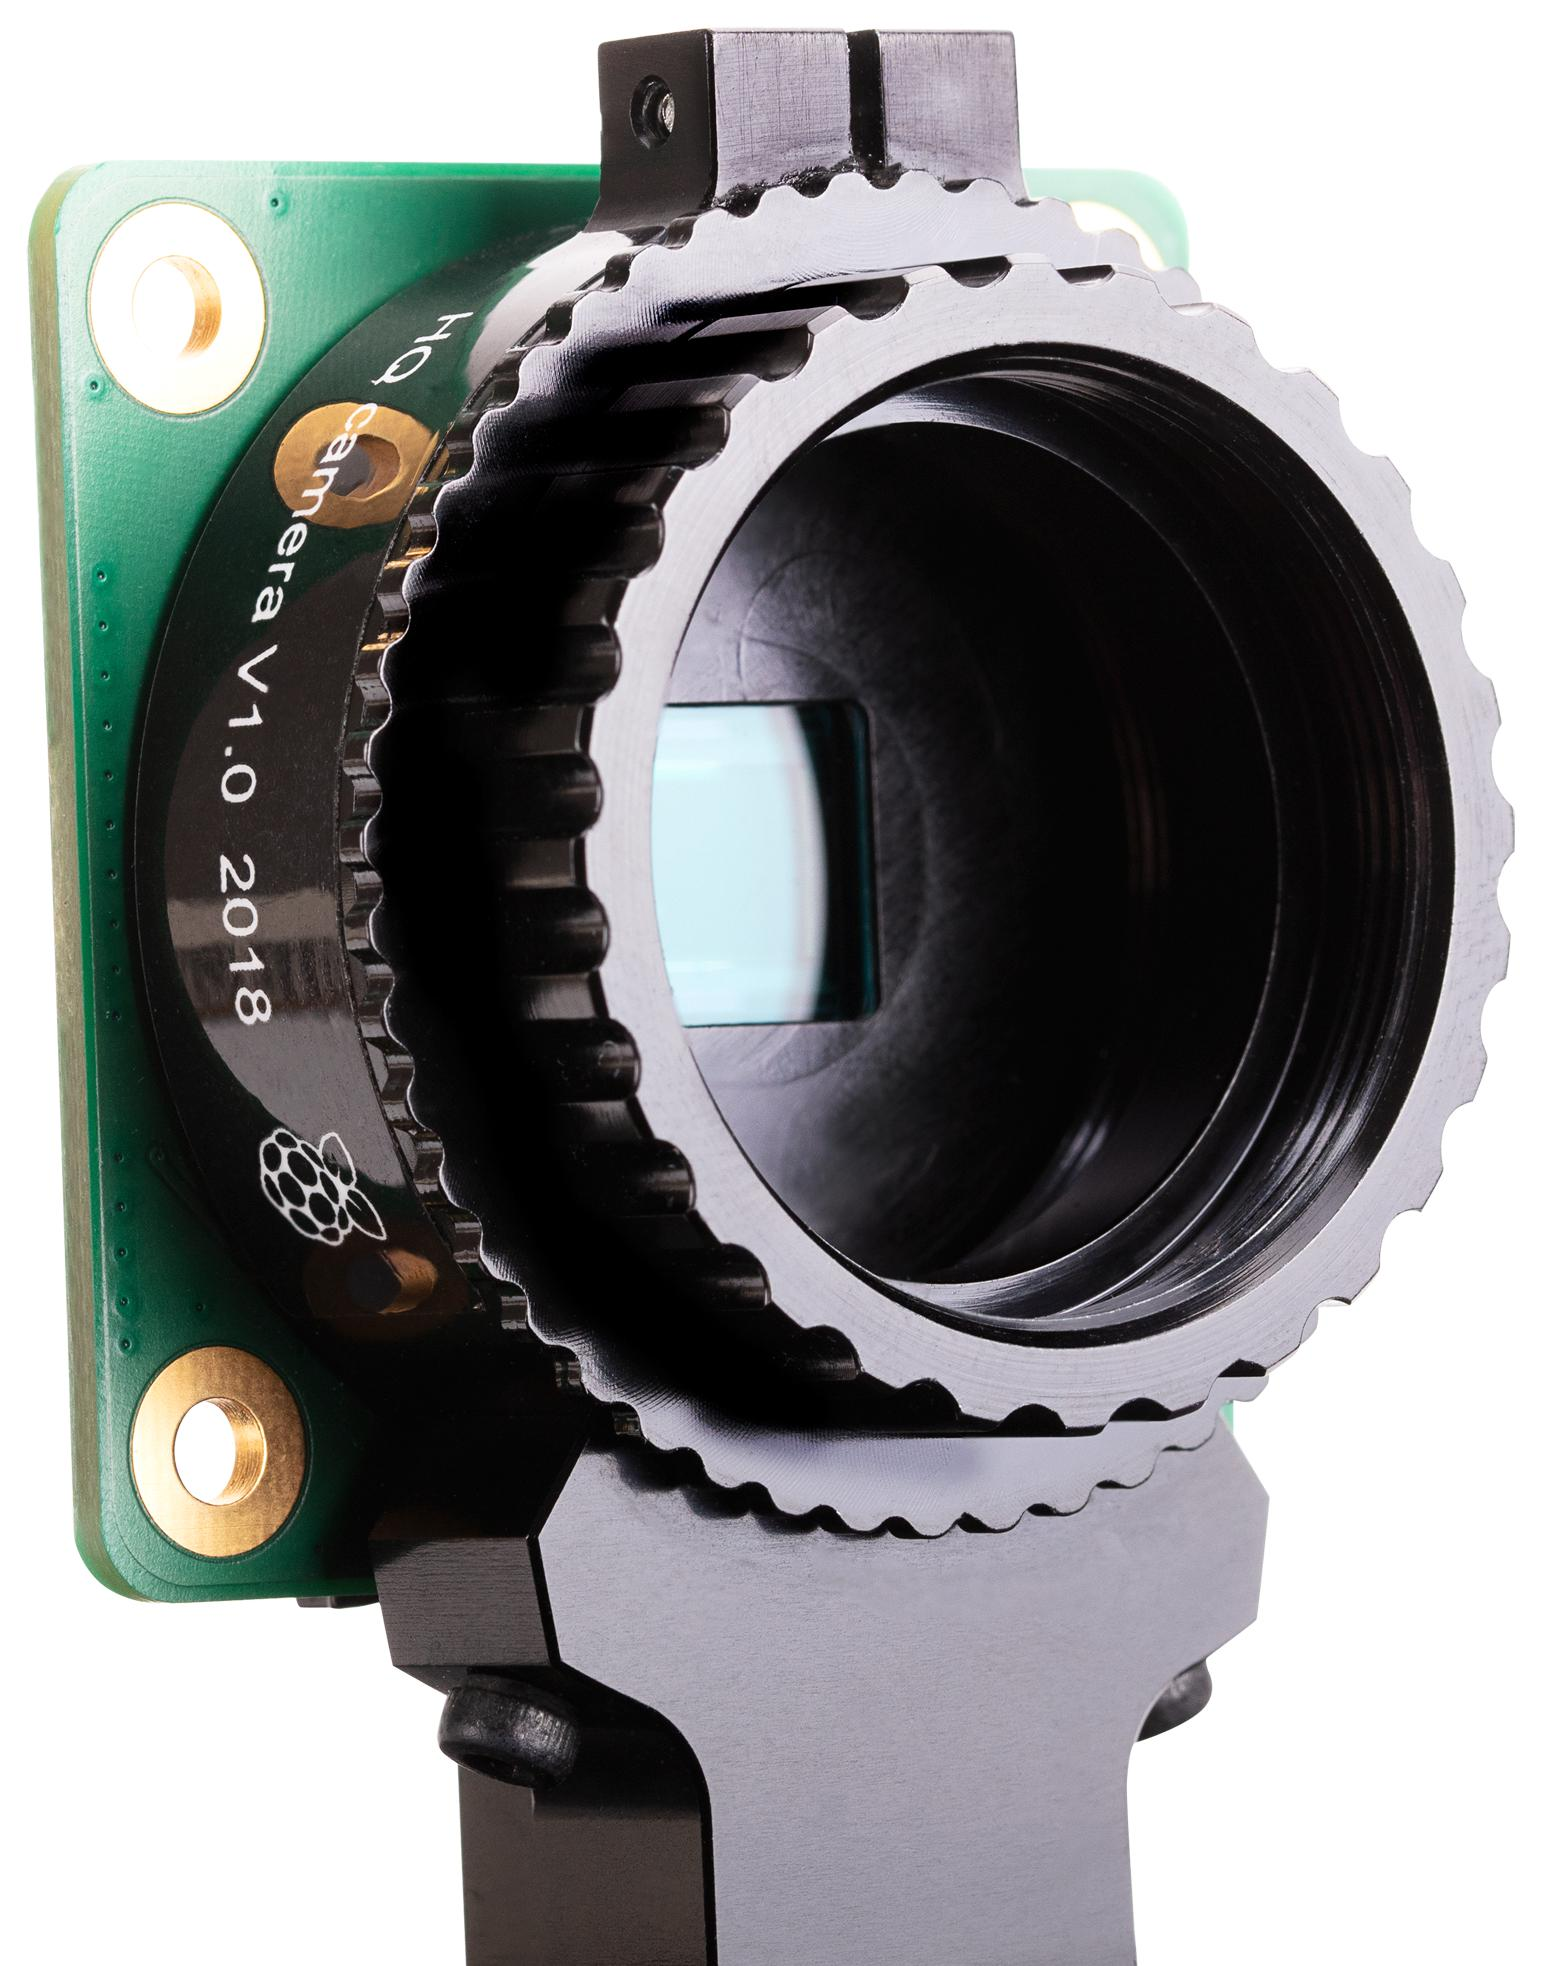
\includegraphics[scale=0.1]{szenzor.jpg}
    \caption{Optikával és optika nélkül felszerelt RPi HQ kamera}
\end{figure}\\

\subsection{Deep Learning}
A deep learning (mélytanulás) a gépi tanulás egy területe, melyben 
neurális hálókat használnak. Rendkívül számításigényes a modellek tanítása, 
de megfelelően komplex hálóval bármilyen függvény közelíthető (létrehozható), 
azaz a nemlineáris klasszifikáció is elvégezhető velük, ezért objektumdetektálásra 
megfelelő architektúrával alkalmasak.
\subsection{Objektum detektálás mélytanulás alapon}
A neurális hálók alapján történő objektum detektálás célja, hogy a neurális 
hálóba beérkező inputból (kép) a háló kimenetén olyan struktúrát kapjunk, mellyel 
leírható az objektumok pozíciója a képen, az alábbi reprezentációk a legnépszerűbbek:
\subsubsection{Bounding box}
A bounding box detection esetében az egyes osztályokhoz tartozó objektumokat 
befoglaló téglalalpokat keresünk a neurális hálóval, ez sokszor elegendő és 
gyorsabb a többi detektálási lehetőségnél.
\subsubsection{Semantic segmentation}
Ebben a szegmentálási típusban minden egyes pixelhez valamilyen osztályt rendelünk, 
ez lehet a háttér (BG) is (komplexebb, magasabb rendű mint a bounding box). Önvezetés témakörében népszerű alaprendszert biztosít.
\subsubsection{Instance segmentation}
Ebben az esetben csak a felismert osztályokhoz tartozó objektumokat reprezentáló 
pixelek kerülnek detektálásra (outputon csak ezeket látjuk).
\subsubsection{Keypoint detection}
A keypoint detection esetében egy képen egyrészt az egyes class-okhoz
tartozó objektumokat szeertnénk detektálni, illetve egy-egy osztálynak
tetszőleges nevezetes pontjait is precízen detektálni szeretnénk. Például 
egy egyszerű rgb kamera által összetett humán mozgások vizsgálata esetén 
gyakran alkalmazzák napjainkban. A projekt szempontjából az orientáció 
és elhelyezkedés könnyedén származtatható ilyen módszerrel.

\subsection{Projekt során nem vizsgálandó hálóarchitektúrák}
Az olyan jellegű ipari feladatoknál, melyeknél egy adott gyártógép/gyártócella kiszolgálása
zajlik valamilyen robottal, kiemelten fontos a precizítás mellett az időhatékonyság, 
azaz jelen esetben, hogy közel valós időben képesek legyünk megállapítani a
munkatérben tartózkodó csatlakozóházakról, hogy milyen típusúak, továbbá felvehetőek-e 
a manipulátorral. Ennélfogva bár mindenképp megvizsgálásra kerül a későbbiekben, de 
első közelítésben nem foglalkozunk olyan hálóarchitektúrákkal, melyek nem képesek közel 
real-time működésre, hiszen ekkor egy olyan nagyságú $\tau$ időkésést adnánk a 
rendszerünknek, mellyel szinte biztosan instabil lenne, azaz olyan módosításokat 
kellene eszközölnünk az egész rendszeren, melyek kompenzálják ezt a hatást. Példaként 
megemlíthető, hogy ekkor meg kellene állítanunk a futószalagot, amelyen az új 
megmunkálandó csatlakozók érkeznek, ez nagyban vissza tudja fogni a termelékenységet, 
időegységre arányosított kihozatalt.
\subsubsection{RCNN és Faster-RCNN}
AZ RCNN hálóarchitektúrák alapját a konvolúciós layer-ek
képzik, melyek a már tárgyalt módon lokális tulajdonságokat, 
pixelek közti tulajdonságokat képesek kinyerni a képből. 
A konvolúciós layer-ek előtt azonban az ilyen architektúrákban 
egy úgynevezett "region extractor" helyezkedik el, 
melynek feladta, hogy a képet kisebb részekre ossza, 
mégpedig olyan formán, hogy olyan régiókat kapjunk, 
melyekben valószínűsíthetően egy-egy objektum helyezkedik 
vagy éppen egy objektum sem helyezkedik el.\\[5pt]
A mélyebb technikai részletektől eltekintve elmondható, hogy 
több megoldás is létezik a régió kinyerésre, de minden esetben 
kétlépéses objektumdetektálásról beszélünk, hiszen 
az objektum klasszifikáció és pixelszintű regresszió 
csak a háló 2. (konvolúciós) részében valósul meg.\\
Ennélfogva mint a többi kétlépéses objektum detektáló háló,
valós időben nem képesek működni, továbbá az RCNN-ek egy sajátossága, 
hogy tanításuk kifejezetten nehézkes főként az adatelőkésztés 
miatt.\\[5pt]
A FASTER-RCNN ahogy azt a név is mutatja egy gyorsabb, 
de még mindig valós időhöz képest lassú hálóarchitektúra.\\[5pt]
Ennélfogva a projekt szerves részét nem képzi az RCNN-ek 
vizsgálata.
\begin{figure}[h]
    \centering
    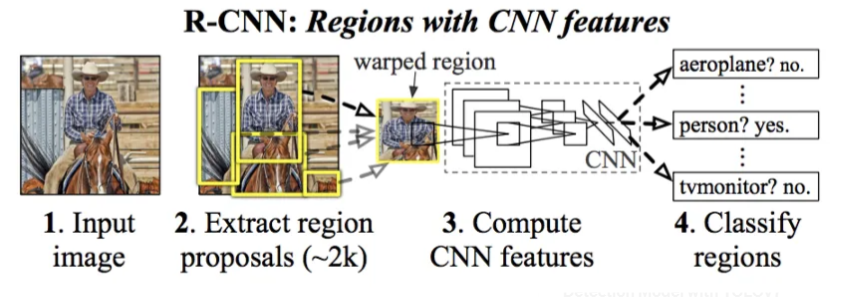
\includegraphics[scale=0.7]{rcnn.png}
    \caption{RCNN hálóarchitektúra sematikus ábra}
\end{figure} 
\subsubsection{Vision - transzformerek}
A deep learning technikákban a transzformerek először a természetesnyelv feldolgozásban 
kerültek kifejlesztésre és alkalmazásra is, majd 
a legtöbb alkalmazási területen megjelent, többet között
a konvolúciós hálókat is jó ideig maguk mögé utasították 
a vision-transzformerek. Az utóbbi időben ismét 
a konvolúciós hálók javára kezd billenni a mérleg. 
A transzformerek működéséről jelen dokuemntumban nem teszünk 
említést, csupán addig a szintig, hogy sebességüknél fogva
az RCNN-hez hasonlóan nem valós időben operálnak.
\begin{figure}[h]
    \centering
    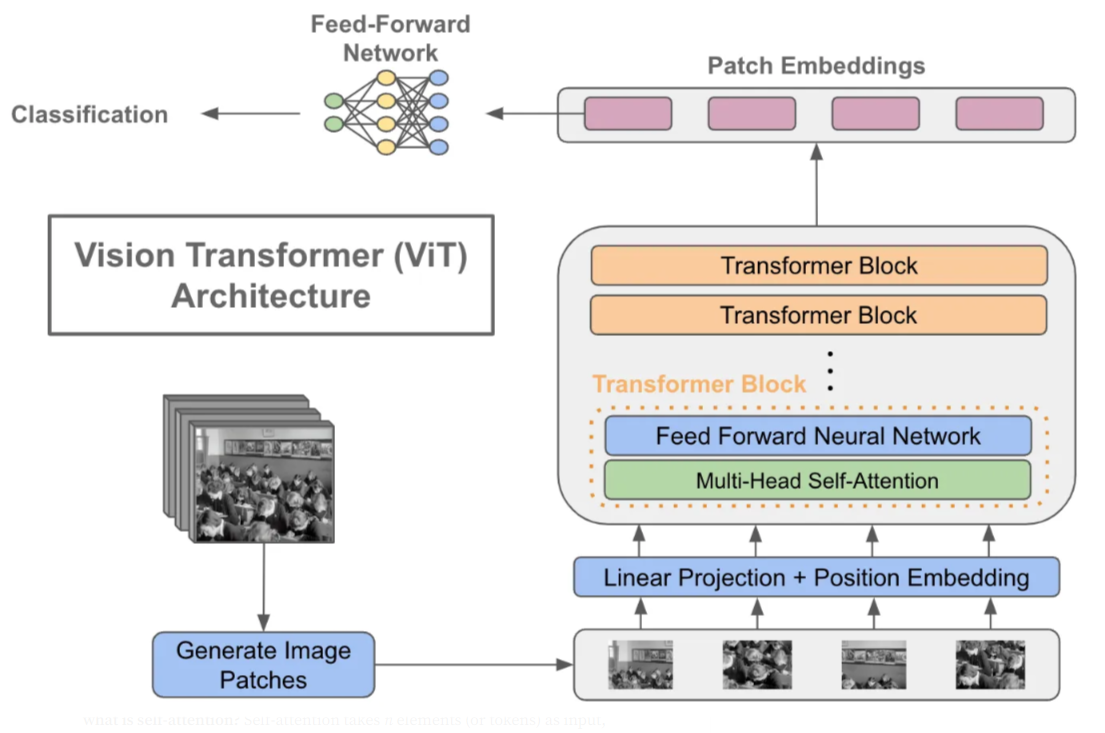
\includegraphics[scale=0.5]{transform.png}
    \caption{Transzformer hálóarchitektúra sematikus ábrája}
\end{figure}

\subsection{Vizsgált hálóarchitektúrák}
\subsubsection{Egyszerű konvolúciós háló - U-net}
Az deep learning alapúobjektumdetektálás egyik legelső implementációja 
az úgynevezett U-net volt, mely konvolúciós layer-ekből áll. 
A bemeneti képet konvolúciós és dropout layereken keresztül 
egy jóval kisebb dimenziójú úgynevezett feature vektorba 
transzformáljuk, majd a háló kiemenete felé közeledve inverz 
transzformációt hajtunk végre a konvolúciós layerekkel, így 
az eredeti kép dimenziójának megfelelő kimenetet kapunk.\\[5pt]
A feature vektorba kódoló részt encodernek, az utána következő 
részt decodernek nevezzük.\\
Belátható, hogy így megfelelő tanítóadattal megoldható 
az objektumdetektálás, azonban szintén észlelhető, hogy 
egyszerűségénél fogva nem feltétlen a legjobb megoldás.\\[5pt]
Sebességét tekintve megfelelően kis paraméterszámmal 
gyors működés érhető el (természetesen a pontosság rovására).
\begin{figure}[h]
    \centering
    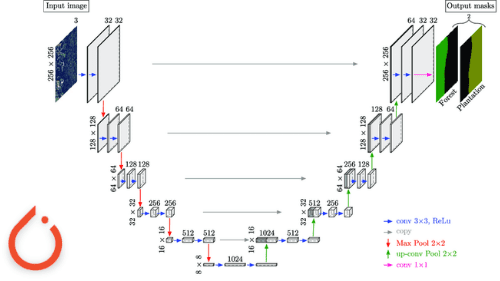
\includegraphics[scale = 0.6]{unet.png}
    \caption{U-net architektúra}
\end{figure} \\
\subsubsection{SSD}
Az SSD (Single-Shot-Detector) egy olyan hálóarchitektúra, mely egy lépésben 
hajtja végre az objektumdetektálást, így lehetséges vele a közel valós 
idejű objektumdetektálás.\\[5pt]
A háló működésének részletes leírására az objektum detektálás dokuemntációban 
kerül sor, röviden az alapgondolat, hogy kisebb, egyenlő nagyságú 
szegmensekre osztjuk a képet, majd ezekre különböző konvolúciós layereket 
hattatva (és azokat a kimenetre csatolva) klasszifikációt hajtunk végre 
(illetve bounding box regressziót természetesen). Mindez egy lépésben történik.\\[5pt]
A YOLO hálóarchitektúra megjelenéséig (illetve a YOLOv2 előtt) a leggyorsabb 
és mellette igen precíz hálóarchitektúrának számított, napjainkban a 
YOLO jobban teljesít.
\subsubsection{YOLO}
A YOLO (You only look once) napjaink egyik, ha nem a legelterjedtebb 
hálótípusa ha objektumdetektálásról van szó. A részletesebb elemzés, illetve 
a későbbiekben a pozíciómeghatározás problémaköre ezen hálóra való illesztése 
az objektum detektálási dokumentációban szerepel. Röviden működését tekintve 
hasonló az SSD-hez hiszen szintén egy lépésben történik a detektálás, továbbá
szintén kisebb szegmensekre osztja az eredeti képet. A fő különbség a két 
módszer között, hogy a YOLO esetében a klasszfikáció regresszióra van visszavezetve, 
hiszen valószínűségi alapon történik a bounding box detektálása (részletesebben lásd obj. detektálás dokumentáció).\\[5pt]
A YOLO-ból évente, de az utóbbi időben akár pár havonta újabb verziók 
érkeznek, melyek egyre jobb és jobb eredményeket adó hálókat eredményeznek.\\
A projekt során főként ezen hálóarchitektúrára fókuszálunk gyorsasága, precizítása 
és nagyfokú generalizáló hatása miatt.
\begin{figure}[h]
    \centering
    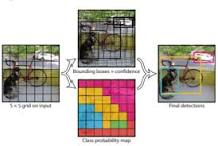
\includegraphics[scale=1]{yolo.jpg}
    \caption{YOLO architektúra működése sematikusan}
\end{figure}\\
\subsection{Konklúzió}
Egyelőre mindösszesen irodalomkutatásra és igen minimális méretű
adathalmazra alapozva mondhatjuk, de mindenképp valós idejű és jól 
általánosítható, precíz hálóra van szükségünk a feladat elvégzéséhez, így 
a különböző YOLO verziók tezstelése, módosítása, kiegészítése egy célravezető 
útnak mutatkozik.

\section{Robot manipulátor}
\subsection{Végberendezés kiválasztása}
Végberendezések tekintetében a lehetőségek feltárását követően 
arra jutottunk, hogy vákuumos megfogókat fogunk alkalmazni, 
hiszen ezek megfelelően egyszerűek és mindösszesen 
három koordinátából determinálható a pozícionálás velük.

\subsection{Modellezés}
A dokumentum által tárgyalt időszakon belül a használt SCARA robot gépészeti modellezése, jellemző adatainak, melyek
a későbbiekben a szimulációknál, digitális ikernél releváns adatként szolgálhatnak, adatlapból és mérésekből történő 
meghatározása, CAD modell elkészítése, illetőleg a gyártócella hasonló megfontolások alapján történő modellezése 
is megtörtént.\\
(képek...)
\begin{figure}[h]
    \centering
    % na ide jönne mindenféle kép de .stepben egyik alkatrészt sem nyitja meg...
    %\includegraphics[scale = 0.5]{robot.png}
    \caption{CAD modellek}
\end{figure}


\section{Irodalomjegyzék}







\end{document}